\thispagestyle{empty}
\begin{center}
    \vspace*{1cm}
    {\huge \bfseries Abstract\par}
    \vspace{1cm}
\end{center}


Il presente documento illustra la progettazione, lo sviluppo e il \textit{deployment} di \textbf{Scalamarket}, una piattaforma e-commerce basata su una moderna architettura a microservizi. L'obiettivo del progetto è di implementare un'architettura a microservizi sufficiente per una piccola attività commerciale, con la possibilità di espandersi in più filiali, e come questo possa essere effettuato attraverso molteplici approcci. In una prima parte ci si focalizzerà sulle componenti dell'ecosistema, formato da Frontend, Auth Service, Inventory Service, Order Service, interfacciati con database PostgreSQL, gestiti mediante orchestrazione \textbf{Kubernetes (K3s)} in un implementazione locale. Viene inoltre analizzato il processo di \textit{provisioning} dell'infrastruttura cloud tramite \textbf{Terraform} su \textbf{Amazon Web Services (AWS)}, con particolare attenzione alle dinamiche di bilanciamento del carico (\textit{Application Load Balancer}) e di instradamento (\textit{Ingress Controller}), impostando anche dei limiti di budget. La relazione documenta l'evoluzione architetturale, partendo da un'impostazione locale essenziale, fino ad arrivare a una topologia orientata all'alta affidabilità (\textit{High Availability}), concludendosi le rotte API utilizzate e come il progetto può essere portato avanti in futuro.

\vspace{1cm}
\begin{figure}[H]
    \centering
    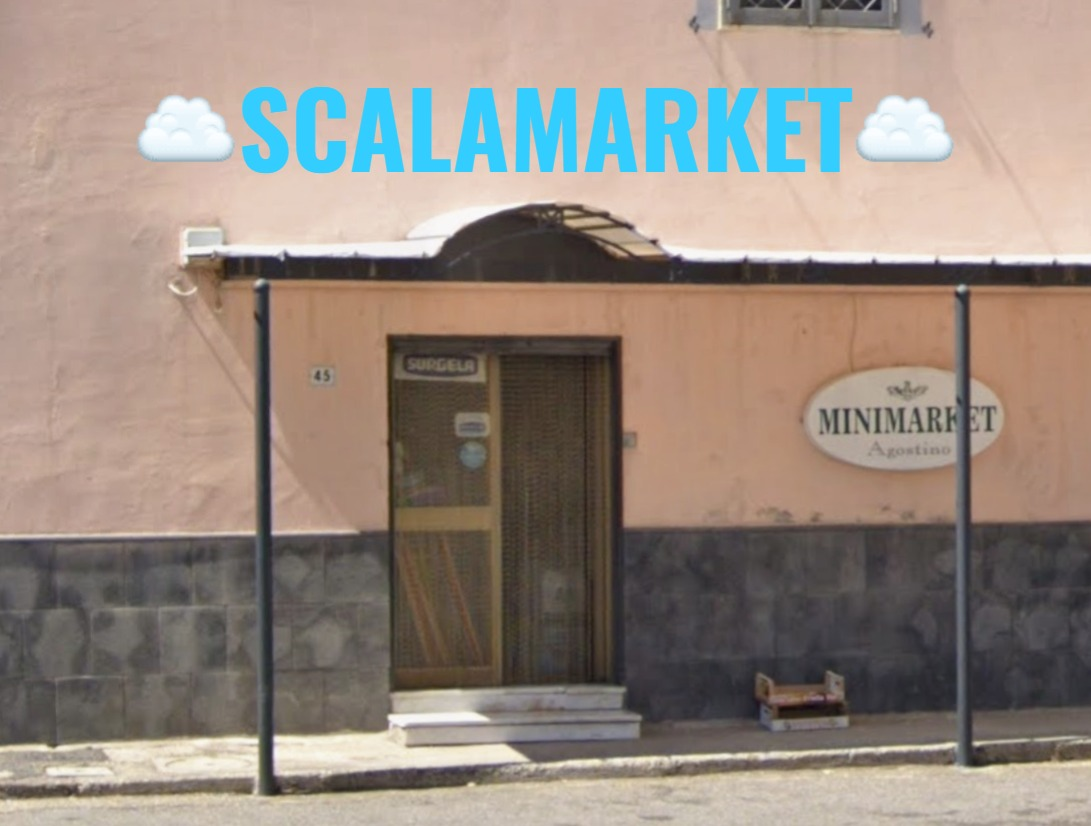
\includegraphics[width=0.5\textwidth]{img/Scalamarket.jpg}
    \caption{Logo di Scalamarket, ispirato principalmente da un minimarket di proprietà della famiglia di un amico}
    \label{fig:scalamarket_logo}
\end{figure}

\clearpage
\cleardoublepage
